In this chapter, state-of-the-art methods of topics related to this thesis are presented in short. At the end of each section, the approach followed in this thesis is positioned with respect to state-of-the-art methods.

\section{Data Mining and Data Extraction from Knowledge Graphs}
The semantic web provides large linked open data sources, which try to connect large amounts of data crawled from the web into a knowledge graph. For example there is \emph{DBpedia} \cite{mendes2012dbpedia} and \emph{Wikidata} \cite{van2019wikidata}. \emph{DBpedia} is a community-based project, that automatically extracts and combines multi-lingual data from Wikipedia into a single knowledge graph. Therefore Wikipedia info boxes are exploited as a source of structured data. In comparison, \emph{Wikidata} is a knowledge graph directly associated with the Wikimedia project (i.e., including Wikipedia) aiming to provide ``[...] universal identifier for all relevant named entities''\cite{van2019wikidata} in an approach to get the central authority for this purpose.

It is necessary to extract the data first to make this kind of data usable with standard machine learning approaches. Narasimha et al. \cite{narasimha2011liddm} proposed a data mining system for linked data called \emph{LiDDM}. \emph{LiDDM} is a model that offers a GUI conducted pipeline to extract linked data from different sources and make it usable for statistical analysis; with results visualized in the end. For data extraction, the user can choose between specifying the SPARQL query and an automatic query builder based on predicate recommendations. The user is only needed to specify the triples.
Cheng et al. \cite{cheng2011automated} provide a theoretical framework to automatically query semantic feature vectors from a knowledge graph based on SPARQL. Given a set of entities $\mathcal{E}$ of interest, they automatically propose a feature vector $v_e \in \{0,1\}$ with semantic neighborhood information for all $e \in \mathcal{E}$.
Moghaddam et al. \cite{moghaddam2021literal2feature} proposed a framework capable of automatic feature extraction from a knowledge graph by generating SPARQL queries based on traversing an RDF graph. Like Cheng et al., they start with a set of entities of interest but aim to retrieve literals instead of a lengthy binary vector automatically.
This thesis uses SPARQL queries like the ones generated by the frameworks above. The user can use any of the tools to generate the query and extract the dataset automatically. The approach won't be dependent on how the SPARQL query to retrieve the dataset is designed. The concept of entities of interest will be formalized because, during the extraction of the dataset, these entities will be aligned with the samples in the extracted dataset. Therefore not only using the knowledge graph as a data source but also as a source for the semantic context of the samples in the dataset, which stays usable after data extraction.

\section{Integrity Constraint Validation}
Cormen et al. \cite{corman2018semantics} introduced the semantics for recursive SHACL and provided complexity bounds for the general problem of SHACL constraint validation over a knowledge graph. In general, the problem turns out to be not solvable in polynomial time, in the case of $P \neq NP$. However, they identified tractable fragments of the language \cite{corman2019validating} and proposed SHACL2SPARQL \cite{corman2019shacl2sparql} an algorithm to tackle these fragments. Nevertheless, the execution of SHACL validation over large knowledge graphs stays expensive, which is why Figuera et al. \cite{figuera2021trav} presented Trav-SHACL. Trav-SHACL is a SHACL engine built to detect invalid entities early in an approach to maximize the scalability of the engine. Both engines interleave the saturation performed by the SAT solver (see section \ref{background_shacl}) with the materialization and grounding of the rules. However, Trav-SHACL rewrites 
the queries sent to the SPARQL endpoint (e.g., pushing \uri{FILTER} terms into the queries to make them more selective). Furthermore, Trav-SHACL chooses the shape validation, such that the shapes, that can invalidate the most number of entities, are validated first. This thesis depends on the performance of SHACL validators and proposes heuristics to minimize the time spent performing SHACL constraint validation. Compared to Trav-SHACL, the heuristics used for optimization will be agnostic to the SHACL engine, enabling the wider application.


\section{Model-agnostic Interpretabilty Methods}
Model-agnostic interpretability methods can be applied in an approach to make black-box models better interpretable. On the one hand, there are global methods to analyze how features influence the prediction of a machine learning model on average (e.g., Partial Dependence Plot \cite{friedman2001greedy}, Accumulated Local Effects Plot \cite{apley2020visualizing}), to measure the feature importance (e.g., model reliance \cite{fisher2019all}) or to build another approximating model, which can be interpreted more easily. 

For example, given a dataset $D$ having the feature set $Z = \{f_1,f_2,...,f_M\}$ the Partial Dependence Plot shows the marginal distribution of the predictions of a machine learning model $M_\theta$ given a subset of the features $Z_C \subset Z$. The marginalization is done by taking the average prediction (in the case of regression) and the most mentioned class (in the case of classification) per $Z_C$ feature combination. This allows seeing the general influence the features in $Z_C$ have on $M_\theta$. 

On the other hand, we have local methods to explain specific predictions of a model like LIME \cite{ribeiro2016should}. Again one might assume a trained machine learning model $M_\theta$, but now one is just interested in the approximate linear effect the features have on the prediction at a given problem instance $\mathbf{x_i}$. Therefore a new dataset $D_2$ for supervised machine learning is generated by varying the feature values of $\mathbf{x_i}$ and for each problem instance generated ask for $M_\theta(\mathbf{x_i} + s_j)$. The $s_j$ ($j \in [1,...,|D_2|]$) might be estimated by sampling $|D_2|$ times from a multivariate normal distributed random variable with zero mean and a covariance matrix $\epsilon * \mathcal{I}$ where $\epsilon > 0$ and $\mathcal{I}$ the identity matrix with dimension $|\mathbf{x_i}| \times |\mathbf{x_i}|$.
Now $|D_2|$ can be used to train an easily interpretable model, which approximates $M_\theta$ at $\mathbf{x_i}$ locally. For instance, in the case of continuous feature and target values, a linear regression $M_w(x) = w * x$ can be used. The weights $w$, as well as the standard deviation of the weights $w_{std}$, can be estimated an interpreted as a feature importance vector $\frac{w}{w_{std}}$.

Both methods help investigate the features' importance when making a prediction with $M_\theta$ for $\mathbf{x_i}$.

However, both examples and the other usual interpretable methods named above have one major drawback: They try to explain the model only with respect to the features, without considering the semantic context provided by a knowledge graph. Figure \ref{fig:related_work_intepretability_methods} illustrates this drawback. The entities of the real world can be captured together with their semantic context in a knowledge graph. The dataset is created based on the entities in the knowledge graph, but the extraction process discards the semantic context the knowledge graph provides. An inducer uses the dataset to train a machine learning model (i.e., a black box model), which is then analyzed by the interpretability methods (e.g., global or local) for better interpretability. However, the semantic context the knowledge graph provides is not considered. This thesis proposes a model-agnostic interpretable method. The semantic context is used in the process of the constraint validation to interpret machine learning models (i.e., especially decision trees) better with respect to patterns detected through the constraint validation.

\begin{figure}
    \centering
    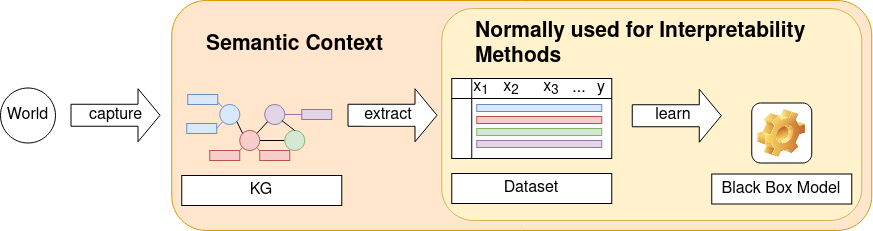
\includegraphics[width=0.8\textwidth]{images/related_work.png}
    \caption{Layers to be considered by interpretability methods: The real world goes through many layers before the interpretability method is used to inform the human about the model. The semantic context is ignored by interpretability methods used normally. (The figure is inspired by \cite{molnar2020interpretable})}    
    \label{fig:related_work_intepretability_methods}
\end{figure}

\section{Explainable Machine Learning over Knowledge Graphs}
Machine learning over knowledge graphs is used for (i) link prediction to identify missing facts (i.e. triples) in the knowledge graph \cite{link_prediction_analysis}, (ii) entity clustering to detect repeating patterns in entities, or even to discover completely synonymous entities \cite{entity_clustering}, (iii) Image Classification \cite{image_classification} and various further applications. All of these approaches somehow make use of the semantic context the knowledge graph provides: Embeddings (e.g., graph-, node-, link embeddings, or messages passed in graph neural networks) incorporate the semantic context and encode it in a latent vector representation. Rule-based approaches yield insights based on the semantic context \cite{rule_based_learning}; for example, in the context of link prediction.

Embedding-based approaches usually scale well with large-size knowledge graphs, but predictions based on them are not inherently explainable. In contrast, when a rule-based approach makes a prediction, it is explainable, since the prediction was made based on a set of rules. Nevertheless, comprehensible rules are usually handcrafted, making these approaches scale worse. 

For example, Halliwell et al. \cite{Halliwell2021} propose using user-scored explanations for rating state-of-the-art model explanations for link predictions. They generate ground truth explanations for links to be rated based on horn clauses. Mohamed et al. \cite{excut} generate explainable labeled clusters based on rule mining. Nevertheless, using embeddings for the task of clustering, the clusters' labels are explainable through they originate from rules. 

In this thesis, the semantic context is exploited by using SHACL constraint validation to make machine learning models' predictions explainable. The explainability, however, originates from using handcrafted rules (i.e., constraints).

\section{Visualization of SHACL constraints}
In the semantic web, the communication and cooperation of machines with humans is a topic \cite{berners2002new}. The visualization of SHACL constraints allows domain experts to understand SHACL constraints without needing them to know RDF Schema (i.e., an RDF vocabulary for data-modeling) and the exact SHACL specification. 

Arndt et al. \cite{visualShapesEditor} propose a graphical RDF Schema editor and visual SHACL editor in a single tool. The tool allows domain experts to create RDF vocabularies and SHACL shape schemas (i.e., SHACL constraints) in a graphical toolbox. The tool is not based on a familiar visual notation. In contrast, Lieber et al. \cite{unSHACLed} present \emph{unSHACLed} a tool, agnostic to the RDF vocabulary used for constraint modeling, that makes use of known visualizations like UML and VOWL. Supporting all common constraint types and editing operations, they were able to reuse familiar notations. In a study with users proficient with Linked Data and UML, 81\% of the questions were answered correctly. However, they could not cover the visualization notation's scalability. A recent master thesis \cite{haneyThesis}, making use of 3D visualization, experimentally studied the effect of the network size based on synthetic shape schemas. It turned out that the number of nodes and links to be rendered had the highest impact on rendering. Nevertheless, up to 5,000 nodes could be rendered in under ten seconds.

This thesis does not visualize SHACL shape schemas. Still, it aims to visualize constraint validation results in a model-coherent way, promoting the interpretability of machine learning models (e.g., decision trees). Therefore a known visualization library (i.e., dtreeviz \cite{dtreeviz}) is adapted, and synthetic shape schemas are used for the evaluation.


\section{Summary}
This chapter presents various topics related to the thesis, supported by current papers. Data extraction is a central topic and will be based on user-defined SPARQL queries. However, the user is free to use automatically generated queries by other frameworks. Constraints exploit the semantic context of entities for an interpretability method based on SHACL validation. The SHACL process will be speed-up by heuristics agnostic to the SHACL engine. When the constraint validation results are available they will be visualized in a familiar way (i.e., familiar to users of dtreeviz). Model predictions are made explainable based on handcrafted constraints.